\section{Caso R e Caso M}
\label{sec:casos}

A extração de resultados seguiu a mesma metodologia nos dois casos: a queda de pressão foi calculada por $\Delta p = \bar{p}_{\mathrm{ent}} - \bar{p}_{\text{saída}}$, com médias de área em $z = 0$~mm e $z = 20$~mm, e os rácios de inchamento na secção final ($z = 60$~mm) por $B_W = x_{\max}/(W/2)$ e $B_H = y_{\max}/H$, com $W/2 = 10$~mm e $H = 1$~mm.

\subsection{Verificação Numérica e Controlo de Coerência Física}
\label{subsec:verificacao}

A estratégia de evolução convergiu com sucesso em ambos os casos ($S = 1$ em 10 passos, sem falhas e com resíduo relativo inferior a $10^{-3}$). A conservação de caudal foi verificada pelo erro $\varepsilon_Q = 0{,}009\,\%$ (Tabela~\ref{tab:verificacao}), correspondente a um fluxo residual numérico de $1{,}8 \times 10^{-11}$~m$^3$/s na superfície livre.

\begin{table}[H]
    \centering
    \small
    \caption{Verificação numérica dos Casos R e M.}
    \label{tab:verificacao}
    \begin{tabular}{lccccc}
        \toprule
        Caso & $|Q_{\mathrm{in}}|$ [m$^3$/s] & $|Q_{\mathrm{out}}|$ [m$^3$/s] & $\varepsilon_Q$ [\%] & Passos (falhados) & Tempo [s] \\
        \midrule
        R & $2{,}000 \times 10^{-7}$ & $1{,}999 \times 10^{-7}$ & 0,009 & 10 (0) & 409 \\
        M & $2{,}000 \times 10^{-7}$ & $1{,}999 \times 10^{-7}$ & 0,009 & 10 (0) & 336 \\
        \bottomrule
    \end{tabular}
\end{table}

A coerência física foi verificada confrontando $\Delta p$ com a solução analítica unidimensional para escoamento desenvolvido de um fluido da lei de potência entre placas paralelas infinitas:
\begin{equation}
    \Delta p_{\mathrm{1D}} = \frac{2L}{h}K\dot{\gamma}_w^n, \quad \text{com} \quad \dot{\gamma}_w = \left(\frac{2n+1}{3n}\right)\frac{6Q_{\mathrm{total}}}{W h^2}.
\end{equation}
Nesta expressão, $h = 2$~mm, $W = 20$~mm, $L = 20$~mm e $Q_{\mathrm{total}} = 4Q = 8 \times 10^{-7}$~m$^3$/s. A formulação analítica fornece $263{,}0$~kPa (R) e $276{,}2$~kPa (M). Os valores do Polyflow ($287{,}4$~kPa e $301{,}5$~kPa) são cerca de 9\,\% superiores devido ao atrito tridimensional introduzido pelas paredes laterais finitas ($W/(2H) = 10$) e ao rearranjo cinemático à saída ($z = 20$~mm). A razão entre casos ($\Delta p_M/\Delta p_R$) é semelhante nos dois métodos: 1,049 no Polyflow e 1,050 na solução analítica, validando a coerência física do modelo.

\subsection{Campos de Escoamento e Deformação do Extrudido}
\label{subsec:resultados}

\paragraph{Queda de pressão na matriz.} A perda de carga calculada no troço confinado ($z \in [0,20]$~mm) foi de $\Delta p_R = 287{,}4$~kPa no Caso R e de $\Delta p_M = 301{,}5$~kPa no Caso M. Para o mesmo caudal imposto de 200~mm$^3$/s no quarto do domínio, o polipropileno (Caso M) exige um acréscimo de pressão de 4,9\,\% face ao fluido de referência.

\paragraph{Distribuição de velocidades.} A Figura~\ref{fig:velocidades} apresenta os mapas de contorno da velocidade no plano médio de simetria ($Y = 0$), com uma escala comum de 0 a 0,035~m/s. Dentro da matriz ($z \in [0,20]$~mm), observa-se um perfil desenvolvido, com velocidade máxima no núcleo central ($X = 0$), atingindo $v_{\max} \approx 0,034$~m/s em ambos os casos e decaindo até zero na parede lateral ($X = 10$~mm). A jusante da aresta de saída ($z > 20$~mm), o núcleo central desacelera e a camada periférica acelera, estabelecendo um escoamento em bloco (\textit{plug flow}) com velocidade aproximadamente uniforme de 0,020~m/s ao longo do jato livre, coerente com o caudal volumétrico e a secção do extrudido.

\begin{figure}[htbp]
    \centering
    \begin{subfigure}[b]{0.48\textwidth}
        \centering
        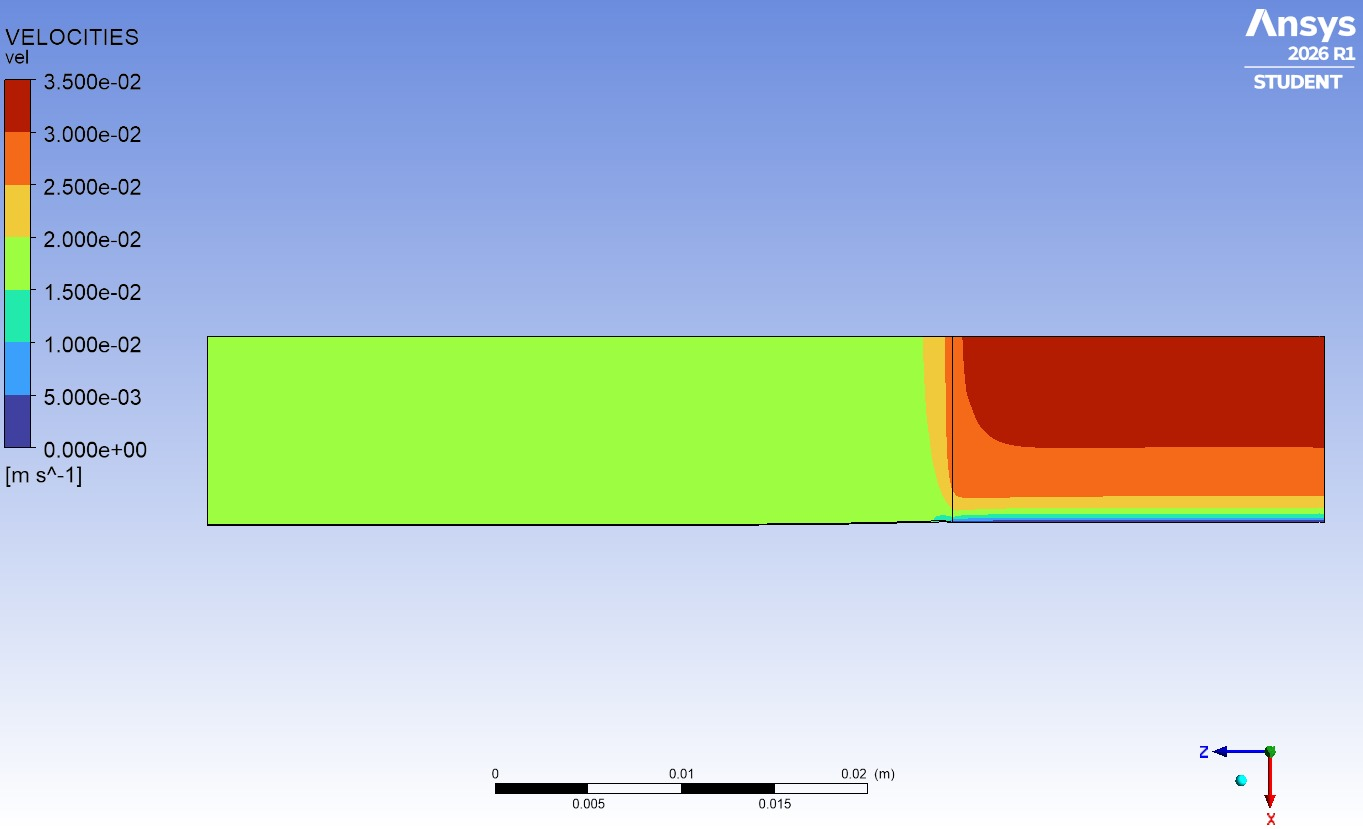
\includegraphics[width=\textwidth]{Imagens/vel_R.jpeg}
        \caption{Caso R (referência)}
        \label{fig:vel_R}
    \end{subfigure}
    \hfill
    \begin{subfigure}[b]{0.48\textwidth}
        \centering
        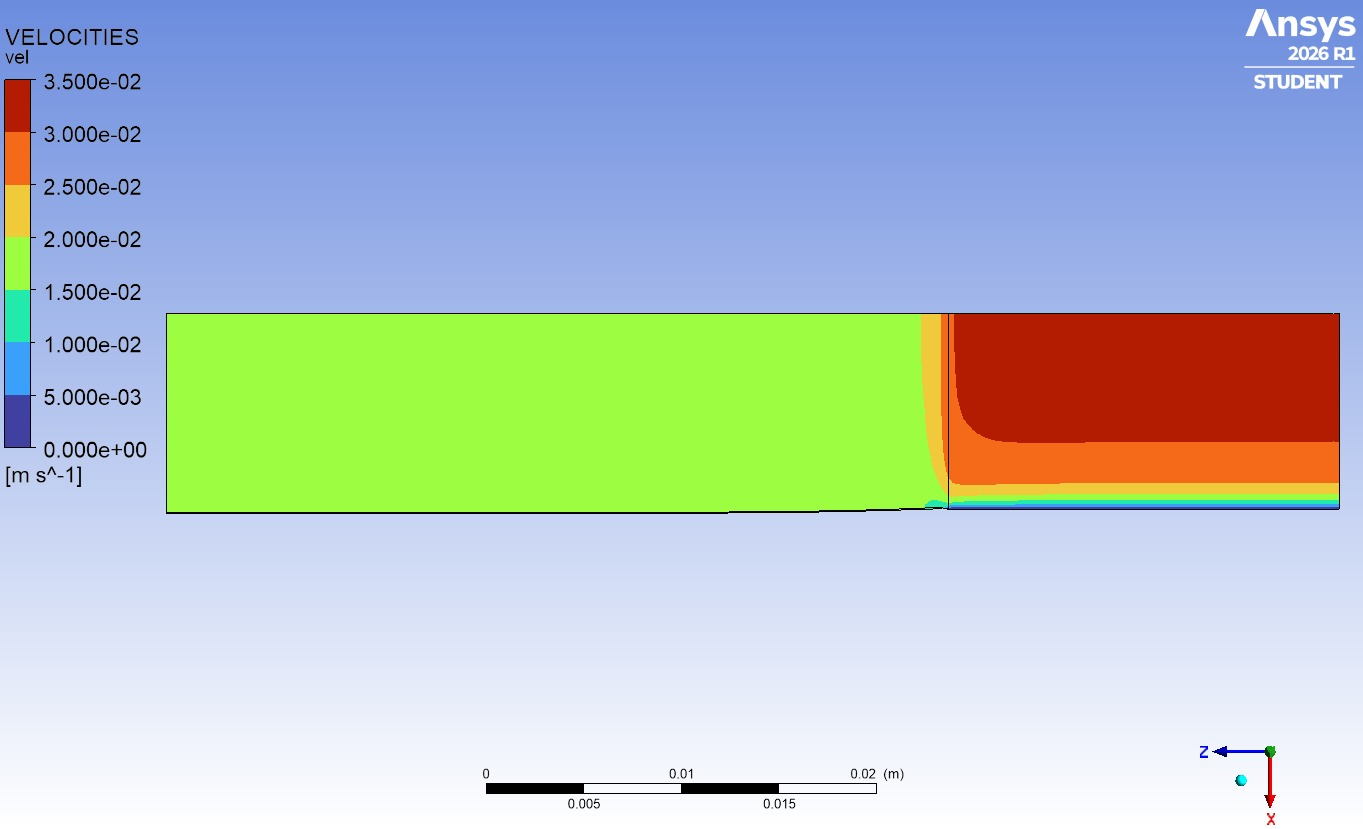
\includegraphics[width=\textwidth]{Imagens/vel_M.jpeg}
        \caption{Caso M (Moplen HP648T)}
        \label{fig:vel_M}
    \end{subfigure}
    \caption{Distribuição de velocidades no plano de simetria $Y = 0$: (a) Caso R e (b) Caso M (escala comum de 0 a 0,035~m/s).}
    \label{fig:velocidades}
\end{figure}

\paragraph{Taxa de deformação.} A Figura~\ref{fig:deformacao} ilustra a distribuição da taxa de corte local ($\dot{\gamma}$) à superfície do domínio, com escala comum de 0 a 90~s$^{-1}$. Na parede da matriz (DIEWALL), a taxa de deformação varia entre 5,5 e 81,5~s$^{-1}$ no Caso R e entre 5,7 e 80,3~s$^{-1}$ no Caso M. O valor médio na secção anterior à saída ($z = 19$~mm) é, respetivamente, 29,1~s$^{-1}$ e 29,3~s$^{-1}$. A aresta de saída da fieira ($z = 20$~mm) constitui a região crítica do domínio, registando-se aí uma descontinuidade abrupta decorrente da transição da condição de não escorregamento para a superfície livre sem tensões. No jato livre, a uniformização do perfil anula os gradientes espaciais de velocidade, fazendo a taxa de deformação decair rapidamente para zero ($\dot{\gamma} \approx 0$~s$^{-1}$).

\begin{figure}[htbp]
    \centering
    \begin{subfigure}[b]{0.48\textwidth}
        \centering
        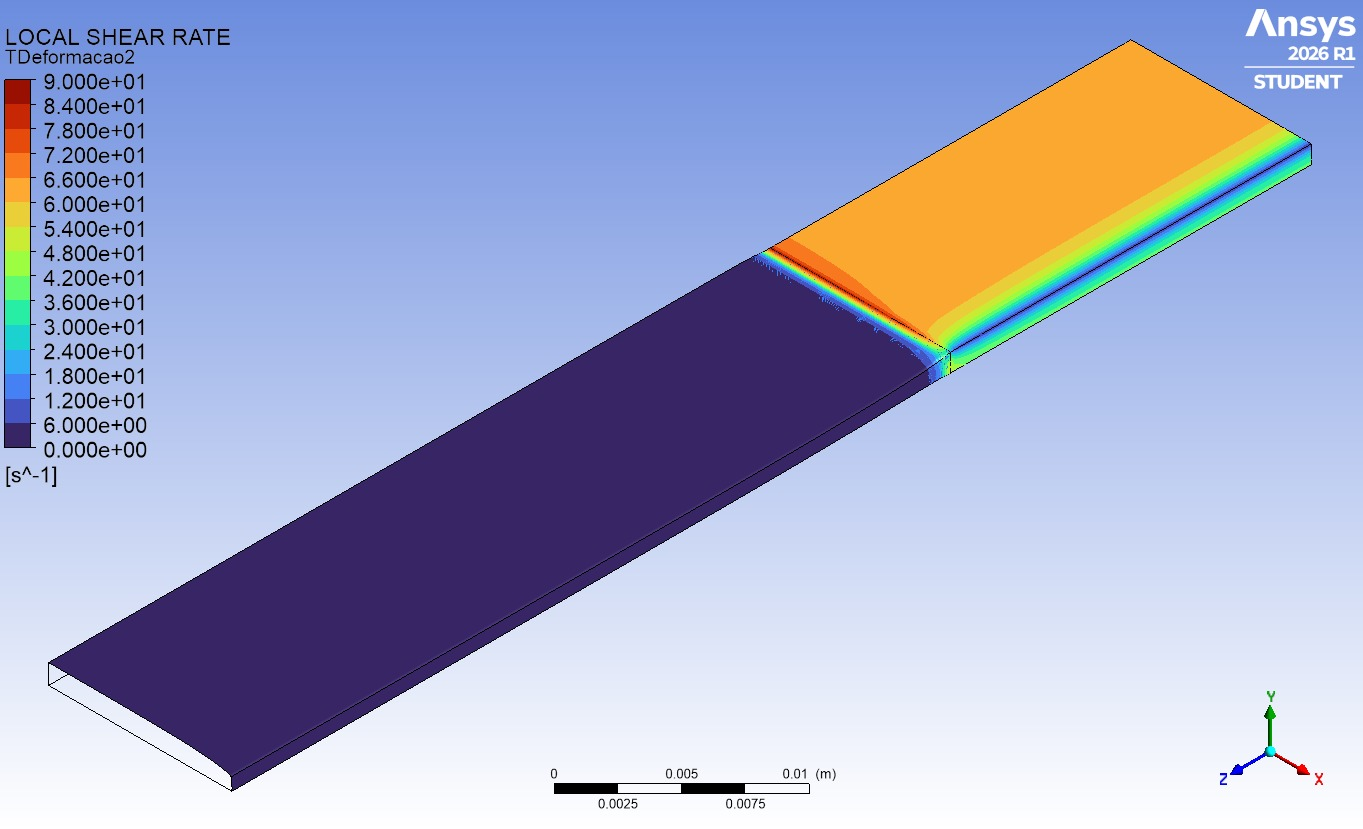
\includegraphics[width=\textwidth]{Imagens/shear_R.jpeg}
        \caption{Caso R (referência)}
        \label{fig:shear_R}
    \end{subfigure}
    \hfill
    \begin{subfigure}[b]{0.48\textwidth}
        \centering
        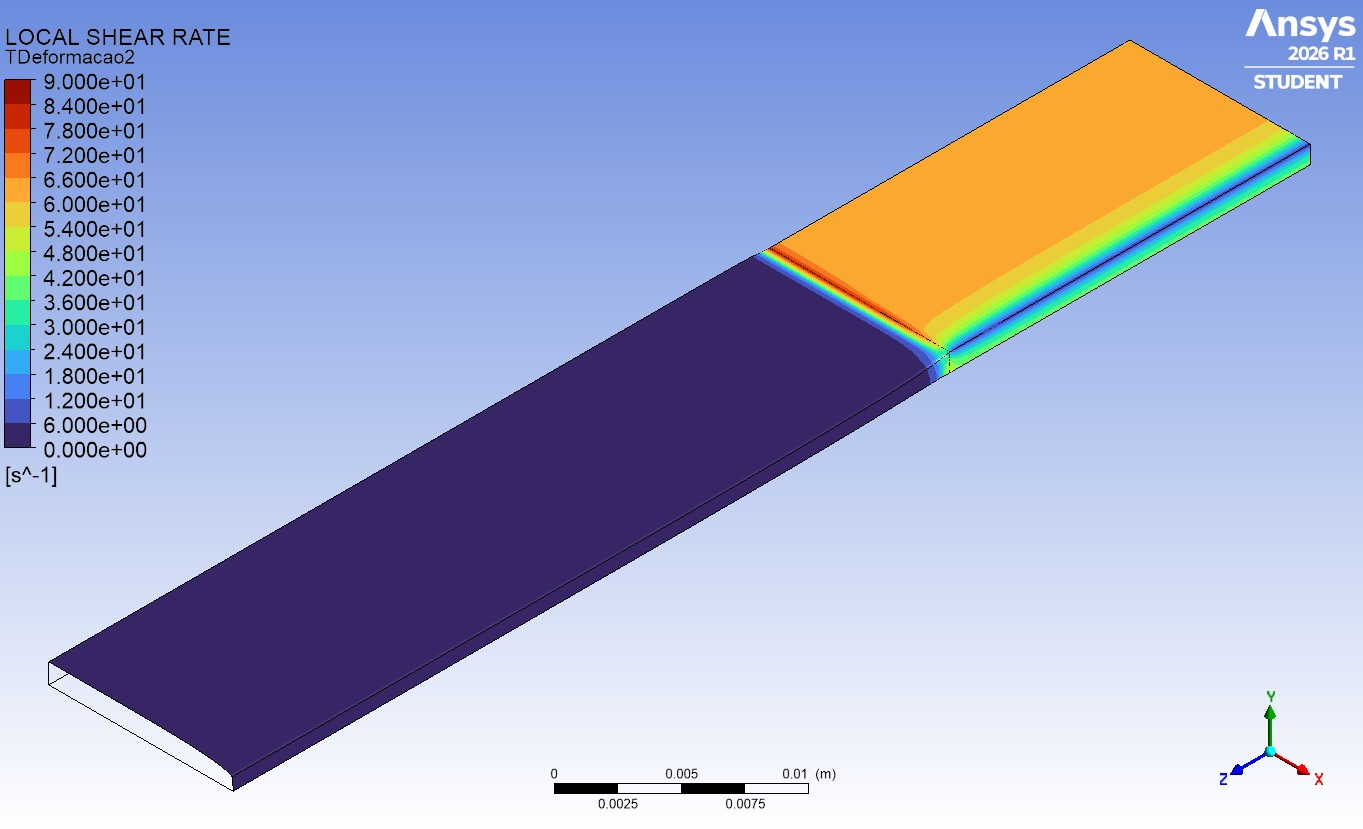
\includegraphics[width=\textwidth]{Imagens/shear_M.jpeg}
        \caption{Caso M (Moplen HP648T)}
        \label{fig:shear_M}
    \end{subfigure}
    \caption{Distribuição da taxa de deformação local ($\dot{\gamma}$): (a) Caso R e (b) Caso M (escala comum de 0 a 90~s$^{-1}$).}
    \label{fig:deformacao}
\end{figure}

\paragraph{Deformação geométrica do extrudido.} A Figura~\ref{fig:inchamento} compara a geometria da secção transversal na saída livre ($z = 60$~mm) com a secção nominal da fieira ($10$~mm $\times 1$~mm). Na secção final, mediram-se os rácios de inchamento $B_W = 1{,}017$ e $B_H = 1{,}096$ para o Caso R, e $B_W = 1{,}023$ e $B_H = 1{,}110$ para o Caso M. Em ambos os fluidos constata-se um inchamento viscoso fortemente anisotrópico: a expansão na espessura ($B_H - 1$, cerca de 9,6\,\% em R e 11,0\,\% em M) é cerca de cinco a seis vezes superior à expansão na largura ($B_W - 1$, cerca de 1,7\,\% em R e 2,3\,\% em M). O bordo superior apresenta uma curvatura acentuada nos cantos exteriores, associada ao efeito tridimensional das paredes laterais da fieira.

\begin{figure}[htbp]
    \centering
    \begin{subfigure}[b]{0.48\textwidth}
        \centering
        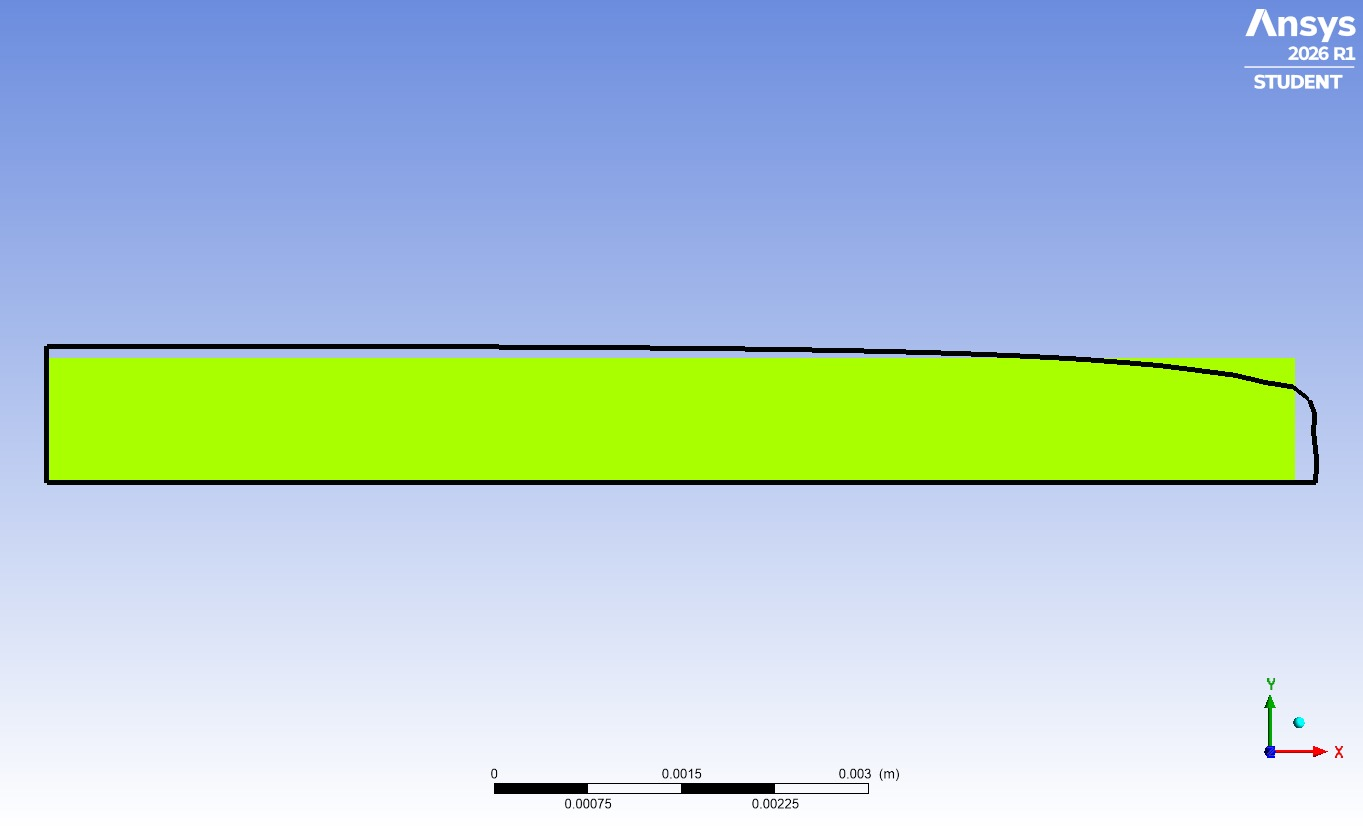
\includegraphics[width=\textwidth]{Imagens/perfil_R.jpeg}
        \caption{Caso R ($B_W = 1,017$; $B_H = 1,096$)}
        \label{fig:perfil_R}
    \end{subfigure}
    \hfill
    \begin{subfigure}[b]{0.48\textwidth}
        \centering
        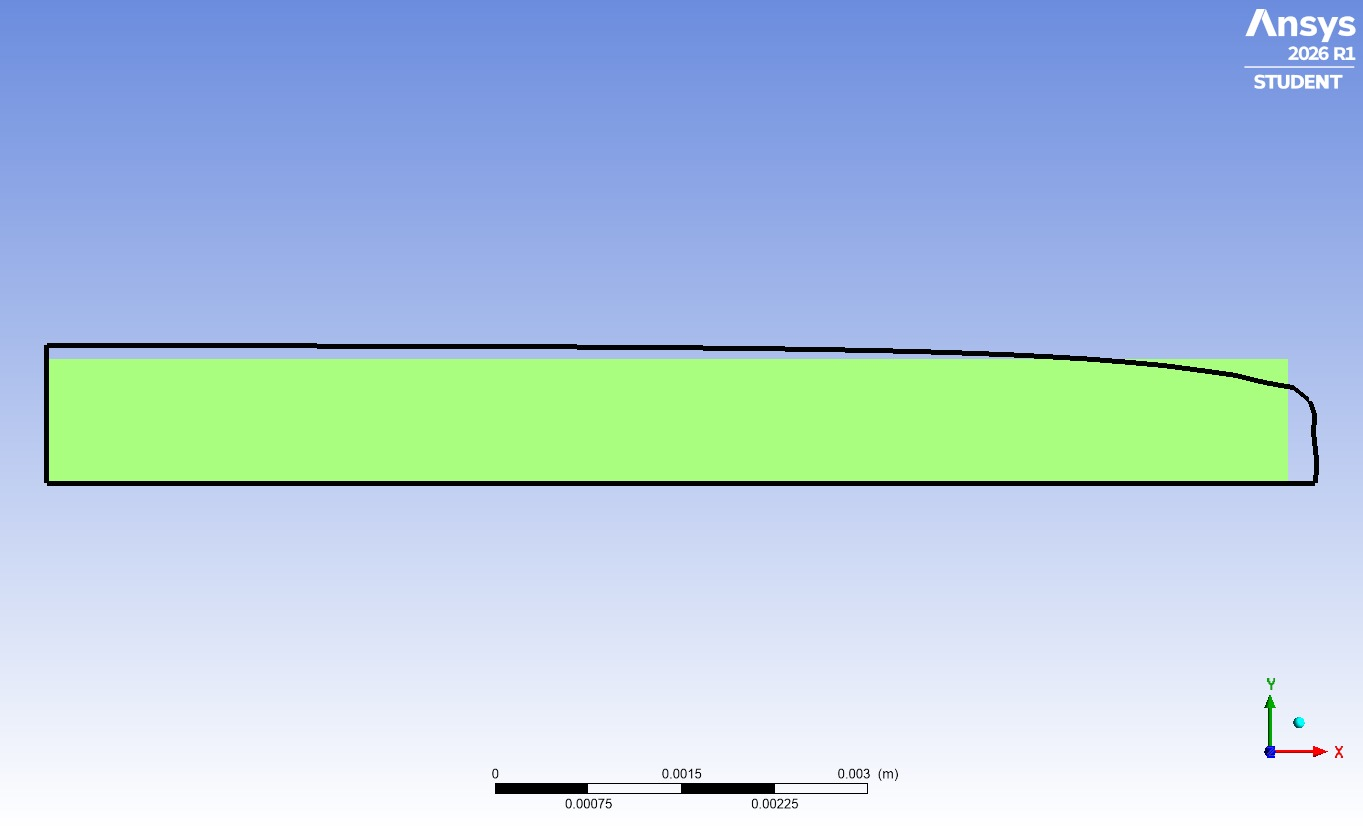
\includegraphics[width=\textwidth]{Imagens/perfil_M.jpeg}
        \caption{Caso M ($B_W = 1,023$; $B_H = 1,110$)}
        \label{fig:perfil_M}
    \end{subfigure}
    \caption{Contorno da secção transversal do extrudido em $z = 60\text{ mm}$ sobreposto à secção nominal da matriz: (a) Caso R e (b) Caso M.}
    \label{fig:inchamento}
\end{figure}

\subsection{Confronto com o Intervalo de Validade da Ficha Reológica}
\label{subsec:validade}

O modelo da lei de potência calibrado para o Moplen HP648T ($K = 900$~Pa$\cdot$s$^n$, $n = 0{,}64$) tem o seu intervalo de validade experimental circunscrito entre 60 e 500~s$^{-1}$, a 220~°C, conforme estipulado na ficha reológica~\cite{FichaMoplen}. A Figura~\ref{fig:validade_ficha} confronta esta janela de calibração com as taxas de deformação calculadas na simulação.

\begin{figure}[htbp]
    \centering
    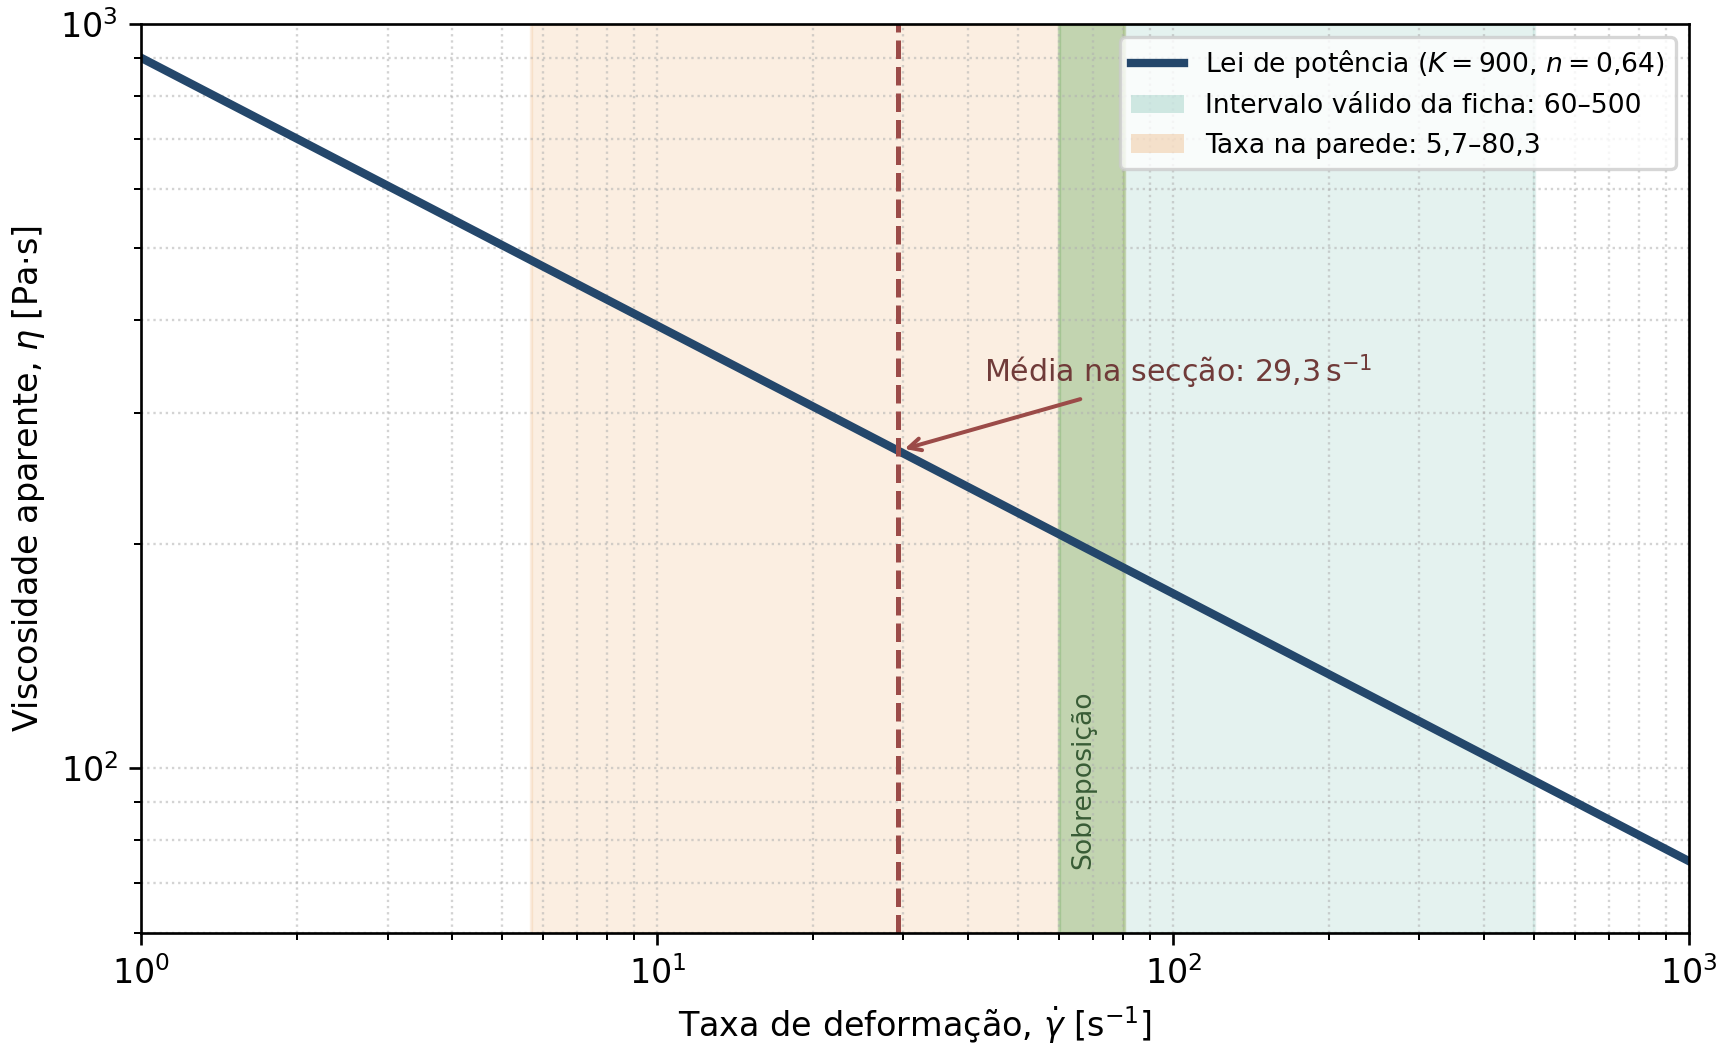
\includegraphics[width=0.72\textwidth]{Imagens/viscosidade_validade.png}
    \caption{Curva reológica do Moplen HP648T a 220~°C e confronto entre o intervalo de validade da ficha e a gama de taxas de deformação obtida no canal da matriz.}
    \label{fig:validade_ficha}
\end{figure}

A taxa de deformação na parede da matriz (DIEWALL) varia entre 5,7~s$^{-1}$, junto aos cantos, e 80,3~s$^{-1}$, no centro da parede larga. O valor médio na secção anterior à saída ($z = 19$~mm) é de apenas 29,3~s$^{-1}$. No núcleo central do canal e ao longo de todo o jato livre, o escoamento tende para velocidades uniformes e $\dot{\gamma}$ decai para valores próximos de zero.

Como se observa na Figura~\ref{fig:validade_ficha}, apenas uma fração estreita do escoamento junto às paredes largas opera dentro do intervalo válido da ficha, entre 60 e 80,3~s$^{-1}$. A maior parte do domínio opera por extrapolação da lei de potência para baixas taxas de corte ($\dot{\gamma} < 60$~s$^{-1}$). Como o modelo puramente potencial não contempla o patamar newtoniano ($\eta_0$), esta extrapolação sobrestima a viscosidade aparente nas regiões de menor cisalhamento, tendendo para $\eta \to \infty$ quando $\dot{\gamma} \to 0$. O limite superior de calibração (500~s$^{-1}$) não é ultrapassado em nenhum ponto do domínio.

\subsection{Quadro Síntese Comparativo (Caso R vs. Caso M)}
\label{subsec:sintese}

Na Tabela~\ref{tab:sintese_RM} apresentam-se e comparam-se as grandezas globais extraídas para o escoamento a caudal imposto ($Q = 2 \times 10^{-7}$~m$^3$/s no quarto do domínio), confrontando o fluido de referência (Caso R) com o polipropileno Moplen HP648T (Caso M). A variação relativa percentual é calculada por $(M-R)/R \times 100\%$.

\begin{table}[H]
    \centering
    \small
    \caption{Síntese dos resultados dos Casos R e M ($Q = 2 \times 10^{-7}$~m$^3$/s no quarto do domínio).}
    \label{tab:sintese_RM}
    \begin{tabular}{lccc}
        \toprule
        Grandeza & Caso R & Caso M & Variação ($M/R$) \\
        \midrule
        $\bar{p}_{\mathrm{ent}}$ [kPa] & 288,0 & 302,3 & $+5{,}0$\,\% \\
        $\bar{p}_{\text{saída}}$ [kPa] & 0,5 & 0,8 & $+53{,}5$\,\% \\
        $\Delta p$ [kPa] & 287,4 & 301,5 & $+4{,}9$\,\% \\
        $\dot{\gamma}_{\max}$ no domínio [s$^{-1}$] & 81,5 & 80,3 & $-1{,}5$\,\% \\
        $\dot{\gamma}$ médio em $z = 19$~mm [s$^{-1}$] & 29,1 & 29,3 & $+0{,}7$\,\% \\
        $\eta$ a $\dot{\gamma}_{\max}$ [Pa$\cdot$s] & 172 & 185 & $+7{,}6$\,\% \\
        $B_W$ [--] & 1,017 & 1,023 & $+0{,}6$\,\% \\
        $B_H$ [--] & 1,096 & 1,110 & $+1{,}3$\,\% \\
        $\varepsilon_Q$ [\%] & 0,009 & 0,009 & -- \\
        \bottomrule
    \end{tabular}
\end{table}

As pressões médias de entrada e saída e as respetivas variações estão arredondadas; os valores de $\Delta p$ e as percentagens foram calculados a partir dos resultados não arredondados.

A comparação da Tabela~\ref{tab:sintese_RM} mostra que a substituição do fluido de referência pelo Moplen HP648T aumenta a perda de carga em 4,9\,\%, acompanhada por um aumento de 7,6\,\% na viscosidade aparente à taxa de deformação máxima. Embora o fator de consistência do Caso M seja inferior ($K = 900$~Pa$\cdot$s$^n$, face a 1000~Pa$\cdot$s$^n$), o seu maior índice de comportamento reológico ($n = 0{,}64$, face a 0{,}60) corresponde a uma menor diminuição da viscosidade com o aumento da taxa de corte. Como $\eta = K\dot{\gamma}^{n-1}$, as viscosidades dos dois materiais cruzam-se perto de $\dot{\gamma} = 13{,}9$~s$^{-1}$: acima desse valor, a viscosidade do Caso M é superior; abaixo dele, a do Caso R é superior. Assim, não se verifica uma viscosidade maior do Caso M em toda a gama de taxas de corte.

Em termos cinemáticos, as taxas de deformação máxima e média permanecem praticamente inalteradas entre os casos (variações de $-1{,}5$\,\% e $+0{,}7$\,\%), indicando que a cinemática global é condicionada sobretudo pela geometria rígida da fieira e pelo caudal volumétrico imposto.

Quanto à resposta geométrica do extrudido, os rácios dimensionais $B_W$ e $B_H$ variam pouco em valor absoluto ($+0{,}6$\,\% e $+1{,}3$\,\%). Considerando o inchamento líquido acima das dimensões da matriz, calculado como $B-1$ a partir dos valores apresentados, a variação do Caso M face ao Caso R é de cerca de $+35$\,\% na largura ($0{,}023/0{,}017 \approx 1{,}35$) e $+15$\,\% na espessura ($0{,}110/0{,}096 \approx 1{,}15$), confirmando a maior propensão do material para a expansão pós-extrusão.